\chapter{Relazioni locali}

Fino a questo momento abbiamo trovato tre equazioni integrali che caratterizzano il campo elettrostatico $\mathbf{E}$

\begin{equation*}
    V_B - V_A = - \int_A^B \mathbf{E} \cdot d \mathbf{s} \quad , \quad \oint \mathbf{E} \cdot d \mathbf{s} = 0 \quad , \quad \oint_{\Sigma} \mathbf{E} \cdot \mathbf{u}_n \ d \Sigma = \frac{q}{\varepsilon_0}
\end{equation*}

Tuttavia è possibile andare a trovare anche una relazione locale che esprime tale equazioni. \\

\' E importante sottolineare che una relazione è locale se, per sapere quanto vale una certa grandezza in un punto $P$, si deve conoscere solo il comportamento delle altre grandezze in quel punto (o in un intorno infinitesimo), non in punti lontani.

\section{Campo elettrostatico come gradiente del potenziale elettrostatico}

Consideriamo l'equazione integrale 

\begin{equation*}
    V_B - V_A = - \int_A^B \mathbf{E} \cdot d \mathbf{s}
\end{equation*}

Andiamo a dimostrare che esiste una relazione locale che permette, dalla conoscenza del potenziale elettrostatico in ogni punto della regione, di calcolare il campo elettrostatico in ogni punto della stessa regione. \\

In \emph{coordinate cartesiane}, per uno spostamento $d \mathbf{s} = dx \ \mathbf{u}_x + dy \ \mathbf{u}_y + dz \ \mathbf{u}_z$ che unisce due punti $A (x,y,z)$ e $B(x+dx, y+dy, z+dz)$ la variazione di potenziale elettrostatico è 

\begin{equation*}
    dV = V(x+dx, y+dy, z+dz) - V(x,y,z) = - \mathbf{E} \cdot d \mathbf{r} = - E_x \ dx - E_y \ dy - E_z \ dz 
\end{equation*}

D'altra parte, per il teorema del differenziale totale

\begin{equation*}
    dV = \frac{\partial V}{\partial x} \ dx + \frac{\partial V}{\partial y} \ dy + \frac{\partial V}{\partial z} \ dz
\end{equation*}

Dal confronto delle due espressioni si ricavano le uguaglianze

\begin{equation*}
    E_x = - \frac{\partial V}{\partial x} \quad, \quad E_y = - \frac{\partial V}{\partial y} \quad, \quad E_z = - \frac{\partial V}{\partial z} 
\end{equation*}

\newpage

Scritto in modo più sintetico 

\begin{tcolorbox}[colback=yellow!10!white, colframe=orange!70!black, boxrule=0.8pt]
\begin{equation}
    \mathbf{E} = - \nabla V
    \label{eq:Campoelettrostatico_come_gradiente}
\end{equation}
\end{tcolorbox}

Dove l'operatore \emph{nabla}, \mkeyword{nabla, coordinate cartesiane} in coordinate cartesiane, è definito come

\begin{equation}
    \mathbf{\nabla } = \frac{\partial}{\partial x} \mathbf{u}_x + \frac{\partial}{\partial y} \mathbf{u}_y + \frac{\partial}{\partial z} \mathbf{u}_z = \colvec{\frac{\partial}{\partial x} \\ \frac{\partial}{\partial y} \\ \frac{\partial}{\partial z}}
\end{equation}

Sostituendo il risultato ottenuto nella \ref{eq:differenza_di_potenziale}
si ottiene un teorema generale del calcolo vettoriale, noto come teorema del gradiente \mkeyword{teorema del gradiente}:

\begin{tcolorbox}[colback=yellow!10!white, colframe=orange!70!black, boxrule=0.8pt]
\begin{equation}
    V_B - V_A = \int_A^B \nabla V \cdot d \mathbf{s}
    \label{thrm:teorema_del_gradiente}
\end{equation}
\end{tcolorbox}

La variazione di una funzione scalare tra due punti $A$ e $B$ è data dall'integrale di linea del gradiente della funzione scalare lungo una qualunque linea che unisca $A$ e $B$. 



\subsection{Superfici equipotenziali}

\mkeyword{superfici equipotenziali}L'andamento di un potenziale elettrostatico è visualizzabile ricorrendo alle superfici equipotenziali definite come le superfici dello spazio tridimensionale nei cui punti il potenziale ha lo stesso valore. \\

Ricordando le proprietà di direzione e verso del gradiente, che ad ogni modo si deducono dalla \ref{thrm:teorema_del_gradiente},

\begin{equation*}
    dV = \nabla V \cdot d \mathbf{s} = - \mathbf{E} \cdot d \mathbf{s} 
\end{equation*}

abbiamo che per uno spostamento $d \mathbf{s}$ tangente a una superficie equipotenziale la variazione $dV$ è ovviamente nulla e quindi il gradiente è ortogonale in ogni punto alla superficie equipotenziale. \\
Inoltre si ha che il campo elettrostatico risulta in ogni punto perpendicolare alla superficie equipotenziale passante per quel punto e il suo verso indica il verso di crescita del potenziale elettrostatico e le superfici equipotenziali sono ortogonali alle linee di forza.



\newpage

\section{Rotore di un campo vettoriale e Teorema di Stokes}

Consideriamo un percorso rettangolare infinitesimo ABCD che giace sul piano \emph{yz} e ha i lati, lunghi $AB = dy$ e $BC = dz$ paralleli agli assi, vogliamo clacolare la circuitazione di un \emph{generico} campo vettoriale $\mathbf{E}$.

\begin{figure} [h]
    \centering
    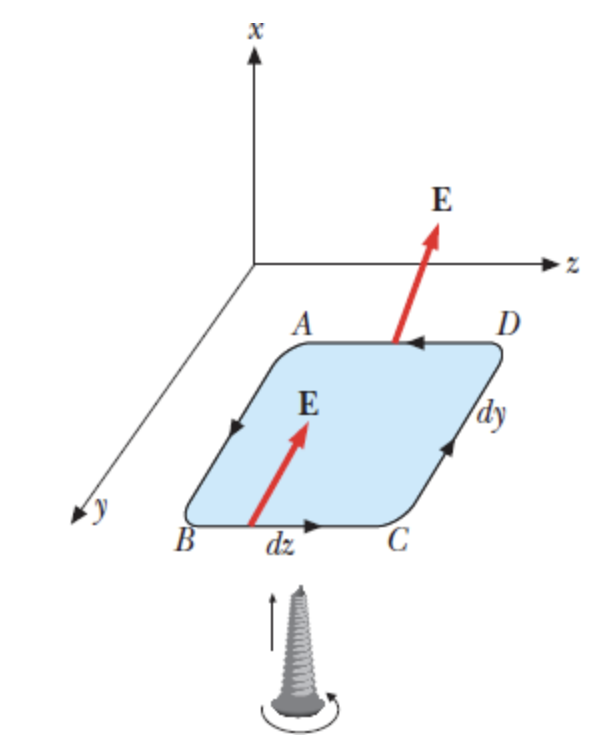
\includegraphics[width=0.5\linewidth]{figure/image2.png}
    \caption{Calcolo della circuitazione di un campo vettoriale $\mathbf{E}$}
    \label{fig:chapter_4_1}
\end{figure}

Il verso di percorrenza è dato dalla \emph{regola della vite destrorsa} \mkeyword{regola della vita destrorsa}, come si vede dal disegno, \emph{ruotando lungo il verso di percorrenza della vita destrorsa, la punta della vite indica il verso dell'asse x}. L'area vale $d \Sigma_x = dy \ dx$.

\begin{equation*}
    d \Gamma_x(\mathbf{E}) = \mathbf{E}(AB) \cdot \mathbf{AB} + \mathbf{E}(BC) \cdot \mathbf{BC} + \mathbf{E}(CD) \cdot \mathbf{CD} + \mathbf{E}(DA) \cdot \mathbf{DA}
\end{equation*}

Dato che $\mathbf{CD} = \mathbf{-AB}$ e $\mathbf{DA} = \mathbf{-BC}$ 

\begin{equation*}
    d \Gamma_x(\mathbf{E}) = [\mathbf{E}(AB) - \mathbf{E}(CD)] \cdot dy \ \mathbf{u}_y + [\mathbf{E}(BC) - \mathbf{E}(DA)] \cdot dz \ \mathbf{u}_z
\end{equation*}

Svolgendo i prodotti scalari e sostituendo le coordinate si ottiene 

\begin{equation*}
    d \Gamma_x(\mathbf{E}) = [E_y(z) - E_y(z + dz)] \cdot dy  + [E_z(y + dy) - E_z(y)] \cdot dz
\end{equation*}

Sviluppando in serie le differenze e fermandosi al primo ordine 

\begin{equation*}
    E_y(z + dz) - E_y(z) = \frac{\partial E_y}{\partial z} dz \quad , \quad E_z(y + dy) - E_z(y) = \frac{\partial E_z}{\partial y} dy
\end{equation*}

Pertanto 

\begin{equation*}
    d \Gamma_x(\mathbf{E}) = (\frac{\partial E_z}{\partial y} - \frac{\partial E_y}{\partial z} ) dy\ dz = (\frac{\partial E_z}{\partial y} - \frac{\partial E_y}{\partial z} ) d \Sigma_x
\end{equation*}

\newpage

Procendendo in modo analogo sui piani $xz$ e $xy$ si ottiene 

\begin{align*}
        d \Gamma_y(\mathbf{E}) = (\frac{\partial E_x}{\partial z} - \frac{\partial E_z}{\partial x} ) d \Sigma_y   \\  d \Gamma_z(\mathbf{E}) = (\frac{\partial E_y}{\partial x} - \frac{\partial E_x}{\partial y} ) d \Sigma_z
\end{align*}

Consideriamo adesso un punto nello spazio e una superficie $d \Sigma $ infinitesima alla quale associamo il vettore $d \Sigma \ \mathbf{u}_n$. Da cui 

\begin{equation*}
    d \Sigma \ \mathbf{u}_n = \colvec{d \Sigma_x \\ d \Sigma_y \\ d \Sigma_z}
\end{equation*}

La circuitazione $d \Gamma$ del vettore $\mathbf{E}$ lungo il contorno $d \Sigma$ è uguale alla somma delle circuitazioni $d \Gamma_x$, $d \Gamma_y$, $d \Gamma_z $, quindi 

\begin{equation}
    d\Gamma(\mathbf{E}) = (\frac{\partial E_z}{\partial y} - \frac{\partial E_y}{\partial z} ) d \Sigma_x + (\frac{\partial E_x}{\partial z} - \frac{\partial E_z}{\partial x} ) d \Sigma_y + (\frac{\partial E_y}{\partial x} - \frac{\partial E_x}{\partial y} ) d \Sigma_z
    \label{eq: circuitazione}
\end{equation}

Dato che il secondo membro dell'equazione ha la forma di un prodotto scalare tra $d \Sigma \mathbf{u}_n$ e un altro vettore, possiamo definire questo secondo vettore come rotore del campo vettoriale \mkeyword{rotore del campo vettoriale} come 

\begin{equation}
     \nabla \times \mathbf{E} = (\frac{\partial E_z}{\partial y} - \frac{\partial E_y}{\partial z} ) \mathbf{u}_x + (\frac{\partial E_x}{\partial z} - \frac{\partial E_z}{\partial x} ) \mathbf{u}_y + (\frac{\partial E_y}{\partial x} - \frac{\partial E_x}{\partial y} ) \mathbf{u}_z
\end{equation}

Che equivale a dire 

\begin{equation*}
     \nabla \times \mathbf{E} = \colvec{\frac{\partial E_z}{\partial y} - \frac{\partial E_y}{\partial z} \\ \frac{\partial E_x}{\partial z} - \frac{\partial E_z}{\partial x} \\ \frac{\partial E_y}{\partial x} - \frac{\partial E_x}{\partial y}}
\end{equation*}

In questo modo la \ref{eq: circuitazione} può essere scritta come 

\begin{equation}
    d \Gamma (\mathbf{E}) = (\nabla \times \mathbf{E}) \cdot d \Sigma \ \mathbf{u}_n
\end{equation}

Possiamo quindi affermare che la circuitazione di un campo vettoriale $\mathbf{E}$ lungo una linea infinitesima nell'intorno di un punto è uguale al flusso del rotore del campo vettoriale $\mathbf{E}$ attraverso un qualunque elemento di superficie $d \Sigma$ che abbia la linea come contorno. \\


Se si estende questo ragionamento \mkeyword{Teorema di Stokes} a un percorso finito si ottiene il Teorema di Stokes  \footnote{Un approfondimento a proposito si trova nell'appendice A in \cite{ElettromagnetismoeOnde}} 

\begin{tcolorbox}[colback=yellow!10!white, colframe=orange!70!black, boxrule=0.8pt]
\begin{equation}
    \oint_C \mathbf{E} \cdot d\mathbf{s} = \int_{\Sigma} (\nabla \times \mathbf{E}) \cdot d \Sigma \mathbf{u}_n
    \label{Teorema di Stokes}
\end{equation}
\end{tcolorbox}


La circuitazione di un campo vettoriale lungo una linea chiusa orientata $C$ è uguale al flusso del rotore del campo attraverso una qualunque superficie $\Sigma$ che abbia $C$ come contorno, orientata concordamente a $C$ con la regola della vite destrorsa. \\
Si nota che nella \ref{Teorema di Stokes} quello a primo membro è un integrale di linea, mentre quello a secondo membro è un integrale di superificie. 

\subsection{Campo vettoriale conservativo}

Se il campo vettoriale, \emph{come nel caso del campo elettrostatico $\mathbf{E}$}, è conservativo, vale 

\begin{equation*}
    \oint \mathbf{E} \cdot d \mathbf{s} = 0
\end{equation*}

perciò la circuitazione è nulla lungo una qualsiasi linea chiusa $\Gamma$, quindi, dovendo essere valida per ogni superficie $\Sigma$ che poggi su $\Gamma$, vale 

\begin{tcolorbox}[colback=yellow!10!white, colframe=orange!70!black, boxrule=0.8pt]
\begin{equation}
\nabla \times \mathbf{E} = 0 
\end{equation}
\end{tcolorbox}

Il campo elettrostatico è un campo il cui rotore è nullo, ovvero un campo irrotazionale.

\newpage

\section{Legge di Gauss in forma differenziale.\\ Divergenza di un campo vettoriale.}

La legge di Gauss nella forma \ref{eq:Legge_di_Gauss} è una legge integrale che lega il flusso il flusso del campo elettrostatico $\mathbf{E}$ attraverso una superficie chiusa a quelle sorgenti del campo che stanno all'interno delle superfici. \\

Dimostreremo adesso che tale legge può essere espressa in forma differenziale tramite una \emph{relazione locale} che lega le derivate del campo in un determinato punto con la denisità della carica $\rho$ in quel punto. \\

Consideriamo un parallelepidedo infinitesimo centrato in $P \equiv (x,y,z)$, con spigoli $dx,dy,dz$ paralleli agli assi e volume $d \tau = dx \ dy \ dz$, che contiene la carica $dq = \rho (x,y,z) d\tau$. 

\begin{figure} [h]
    \centering
    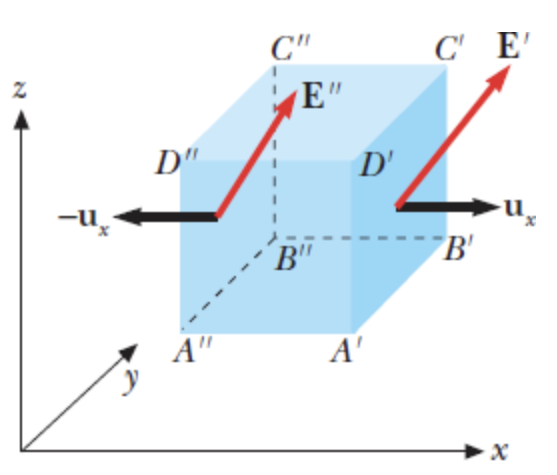
\includegraphics[width=0.5\linewidth]{figure/image11.png}
    \caption{Definizione di divergenza di un campo vettoriale}
    \label{fig:chapter_4_2}
\end{figure}

Il flusso del campo elettrostatico $\mathbf{E}$ attraverso la faccia $A'B'C'D'$, perpendicolare all'asse x, è dato da:

\begin{equation*}
    \mathbf{E}' \cdot \mathbf{u}_x \ dy \ dz = E_x ' \ dy \ dz
\end{equation*}

avendo indicato con $E_x'$ la componente di $\mathbf{E}' = \mathbf{E}\ (x + \frac{dx}{2}, y,z)$ lungo l'asse $x$. Analogamente il flusso attraverso la faccia $A''B''C''D''$ è 

\begin{equation*}
    \mathbf{E}'' \cdot (- \mathbf{u}_x) \ dy \ dz = -E_x '' \ dy \ dz
\end{equation*}

Dove $E_x '' $ è la componente di $\mathbf{E}'' = \mathbf{E}\ (x - \frac{dx}{2}, y,z)$ lungo l'asse $x$. Complessivamente 

\begin{equation*}
    (E'_x - E_x '') \ dy \ dz = \frac{\partial E_x}{\partial x} \ dx \ dy \ dz
\end{equation*}

Espressioni simili si hanno per le altre coppie di superficie e quindi il flusso attraverso tutta la superficie del parallelepipedo è:

\begin{equation*}
    d \Phi (\mathbf{E}) = \mathbf{E} \cdot \mathbf{u}_n \ d \Sigma  = \left ( \frac{\partial E_x}{\partial x} + \frac{\partial E_y}{\partial y} + \frac{\partial E_z}{\partial z} \right ) \ dx \ dy \ dz = \left ( \frac{\partial E_x}{\partial x} + \frac{\partial E_y}{\partial y} + \frac{\partial E_z}{\partial z} \right ) d \tau
\end{equation*}

Poiché, secondo la legge di Gauss \ref{eq:Legge_di_Gauss},

\begin{equation*}
    d \Phi (\mathbf{E}) = \frac{dq}{\varepsilon_0} = \rho (x,y,z) \frac{d \tau}{\varepsilon_0}
\end{equation*}

Quindi otteniamo la relazione locale che cercavamo:

\begin{equation}
    \frac{\partial E_x}{\partial x} + \frac{\partial E_y}{\partial y} + \frac{\partial E_z}{\partial z} = \frac{1}{\varepsilon_0} \rho (x,y,z)
\end{equation}

La combinazione di derivate a primo membro prende il nome di \mkeyword{divergenza del campo $\mathbf{E}$} divergenza del campo $\mathbf{E}$. \\
QUindi vale:

\begin{tcolorbox}[colback=yellow!10!white, colframe=orange!70!black, boxrule=0.8pt]
\begin{equation}
    \nabla \cdot \mathbf{E} = \frac{\rho}{\varepsilon_0}
    \label{eq:Gauss_forma_differenziale}
\end{equation}
\end{tcolorbox}

Il campo $\mathbf{E}$ ha divergenza diversa da zero solo nei punti in cui è diversa da zero la densità di carica. \\

Inoltre si vede facilmente che vale 

\begin{tcolorbox}[colback=yellow!10!white, colframe=orange!70!black, boxrule=0.8pt]
\begin{equation}
    d \Phi (\mathbf{E}) = \nabla \cdot \mathbf{E} \ d \tau
\end{equation}
\end{tcolorbox}

Considerato un volume infinitesimo $d \tau$ nell'intorno di un punto $P$ il flusso del campo vettoriale attraverso la superficie chiusa che delimita $d \tau$ è uguale al prodotto della divergenza del vettore per il volume $d \tau$ stesso. \\

Facendo il passaggio a un volume finito $\tau$ delimitato dalla superficie chiusa $\Sigma$, si ottiene un teorema \mkeyword{teorema della divergenza} generale del calcolo vettoriale noto come teorema della divergenza 

\begin{tcolorbox}[colback=yellow!10!white, colframe=orange!70!black, boxrule=0.8pt]
\begin{equation}
    \oint _{\Sigma} \mathbf{E} \cdot \mathbf{u}_n \ d \Sigma = \int_{\tau} \nabla \cdot \mathbf{E}\ d \tau
\end{equation}
\end{tcolorbox}

\subsection{Equazioni di Poisson e di Laplace}

Poiché nel campo elettrostatico $\mathbf{E}$ vale la \ref{eq:Campoelettrostatico_come_gradiente}, sostituendo nell'espressione \ref{eq:Gauss_forma_differenziale} si ottiene 

\begin{equation}
    \nabla \cdot \mathbf{E} = - \nabla \cdot \nabla V = -\nabla^2 V  = \frac{\rho}{\varepsilon_0}
\end{equation}

Operando in coordinate cartesiane si ottiene 

\begin{tcolorbox}[colback=yellow!10!white, colframe=orange!70!black, boxrule=0.8pt]
\begin{equation}
    \nabla ^2 V = \frac{\partial^2 V}{\partial x^2} + \frac{\partial^2 V}{\partial y^2} + \frac{\partial^2 V}{\partial z^2} = - \frac{\rho}{\varepsilon_0}
    \label{eq:equazione_di_Poisson}
\end{equation}
\end{tcolorbox}

Questa equazione differenziale che lega \mkeyword{Equazione di Poisson}il potenziale alla densità di carica è detta equazione di Poisson. \\

Nello spazio vuoto essa diventa

\begin{tcolorbox}[colback=yellow!10!white, colframe=orange!70!black, boxrule=0.8pt]
\begin{equation}
   \nabla ^2 V = \frac{\partial^2 V}{\partial x^2} + \frac{\partial^2 V}{\partial y^2} + \frac{\partial^2 V}{\partial z^2} = 0
\end{equation}
\end{tcolorbox}

ed \mkeyword{Equazione di Laplace} è detta equazione di Laplace.\\

L'operatore \mkeyword{laplaciano} $\nabla^2 = \nabla \cdot \nabla$, che in coordinate cartesiane si scrive 

\begin{equation*}
    \nabla^2 = \frac{\partial^2}{\partial x^2} + \frac{\partial^2}{\partial y^2} + \frac{\partial^2}{\partial z^2}
\end{equation*}

si chiama laplaciano. 
